\chapter{光电倍增管的性能测试与筛选}
\label{ch:pmt_test}
由于制造工艺的限制,光电倍增管具有很强的个体差异性,即不同管子的性能差异较大。
因此,在光电倍增管大规模应用时,往往要求对每支管子进行详细的测试,以得到它们各自的性能参数信息。
利用这些信息,探测器的研制者可以淘汰性能参数不达标的管子,可以决定管子在探测器整体中的安装位置,可以得到管子的额定工作电压,甚至可以在探测器部署运行后调节其实际工作电压,最终使探测器整体的探测性能达到最佳。

对于PSD所使用的R4443型光电倍增管,Hamamatsu公司对每支出厂的管子进行了基本的性能测试(包括阳极暗电流、长时间稳定性、阴极/阳极的光灵敏度以及阴极/阳极的蓝光灵敏度),并提供了相应的测试结果。
然而,这些测试只在一个工作电压点进行,而且使用的测试条件(连续、强烈的白炽光照射)与R4443在PSD中的实际工作条件(低强度、低频率的脉冲光照射)迥异。
另外,PSD使用双打拿极引出的分压器电路与上述出厂测试使用的标准分压器差别较大,导致R4443的工作状态也不一致。
因此,这些参数信息只能定性地给出各支管子的基本性能,不能作为PSD研制过程的定量参考。

上述因素决定了:需要根据PSD的具体需求,在实验室独立对R4443光电倍增管进行性能参数测试。
为此,我们专门设计并搭建了一套的PMT批量测试平台。
本章对该测试平台进行了介绍,并详细叙述了该平台在R4443光电倍增管的性能测试中的应用以及测试结果。
根据测得的性能参数数据,依据性能最佳的原则,我们进一步对所有管子进行了筛选,选出了可以用于PSD安装的光电倍增管。

\section{PSD对光电倍增管的测试需求}
由于PSD没有参加DAMPE的触发系统,PSD不需要对粒子的入射时间进行测量。
因此,R4443的时间性能参数没有实际的参考价值,无需在实验室对其进行专门的测试。
另一方面,PSD通过测量沉积能量来实现其所有功能(见第\ref{sec:description:psd_principle}节),而光电倍增管的增益是直接影响探测器能量响应的重要参数。
因此,我们的测试主要关注R4443与增益相关的性能参数,这包括Dy8的增益以及Dy5和Dy8间的相对增益(简称Dy58比值)这两个方面。

PSD要求各探测单元模块的能量响应均匀性好于\SI{25}{\percent}。这意味着,需要

高压分组的限制

\section{PMT批量测试平台}
\label{sec:pmt_test:testbench}
PSD的研制过程中涉及大量的PMT测试工作,包括对570支R4443裸光电倍增管的细致性能测试以及在PSD建造过程中将近200个PMT组件的质量测试(详见第\ref{ch:construction}章)。
为了提高工作效率,减轻测试人员的工作负担,我们设计并建造了能够用于PMT大批量测试的专用测试平台。

\subsection{功能与特点}
\label{sec:pmt_test:testbench_functions}
PMT的批量测试是在大型探测器研制过程中经常碰到的工作。
因此,该测试平台虽然是为了DAMPE-PSD项目专门研制的,但我们在设计中充分考虑了该平台的拓展性和可移植性,使得它能够方便地应用于其它项目的PMT测试工作。
该测试平台的主要特点可以归结为如下几点:
\begin{enumerate}
	\item 测试容量大。大型探测器项目动辄涉及成百上千支PMT的测试,如果能够对多支PMT同时进行测试,就可以显著提高工作效率,加快项目进程。该测试平台最大测试容量达到25支PMT,满足大部分项目的测试需求。
	\item 自动化程度高。PMT的细致测试往往涉及不同的性能指标,一次完整的测试需要花费几个小时的时间。这个过程中,需要对大量的仪器设备进行重复操作,如升降高压、切换光强度、移动PMT位置等等。此时,人工操作不仅效率低,而且是不可靠的。因此,该测试平台的关键组件都是用了程控设备,并开发了相应的控制软件,实现了常用设备操的自动化。这样,在PMT的整个测试过程中,人工干预只存在于PMT的安装与卸载,以及相关软件的配置,提高了测试工作的可靠性。
	\item 功能完备。该测试平台能够满足很多潜在的测试需求,即便有些在PSD的研制过程中并不需要。因此,平台使用了一些特殊的硬件模块以及通用的仪器设备。尤其是,我们将三维移动性作为该平台的一个基本功能,使得平台可以用于PMT光阴极的位置扫描。
	\item 扩展性强。测试平台采用模块化设计,其硬件平台是可扩展的,各硬件模块之间的耦合相对松散。这方便了硬件的更换或升级,并可以实现较为复杂的测试方案。软件框架同样基于模块化设计,并对底层硬件进行了虚拟化,使得顶层的测试功能不因底层硬件的改动而有大的变动,增强了测试程序的可移植性。
\end{enumerate}

图\ref{fig:pmt_test:testbench_schematic}给出了PMT批量测试平台的原理框图。
该平台最多可以同时对25支PMT进行测试。光脉冲由一个蓝光LED产生,它经过积分球和集束光纤组成的光分配系统被分成25份,被分别传输到待测PMT的入射端面。
待测PMT都安置在一个固定平台上,而光源和光分配系统被固定在一个三维移动平台上。两个平台相对拜访,这样就实现了对所有待测PMT的光阴极位置扫描。
固定平台上同时安置有两支监控PMT,也接受来自光分配系统的两路入射光脉冲。
在整个测试周期中,两支PMT的位置相对于入射光纤固定不变,因此它们被用于监控LED光源以及整个测试平台性能的稳定性。
这两个支撑平台以及上面的所有测试设备都被放置在一个大小为$176cm\times100cm\times78cm$的铝合金暗箱中(见图\ref{fig:pmt_test:blackbox}),箱子的内壁用黑色图层覆盖以降低内部的杂散光污染。

\begin{figure}[htb]
	\centering
	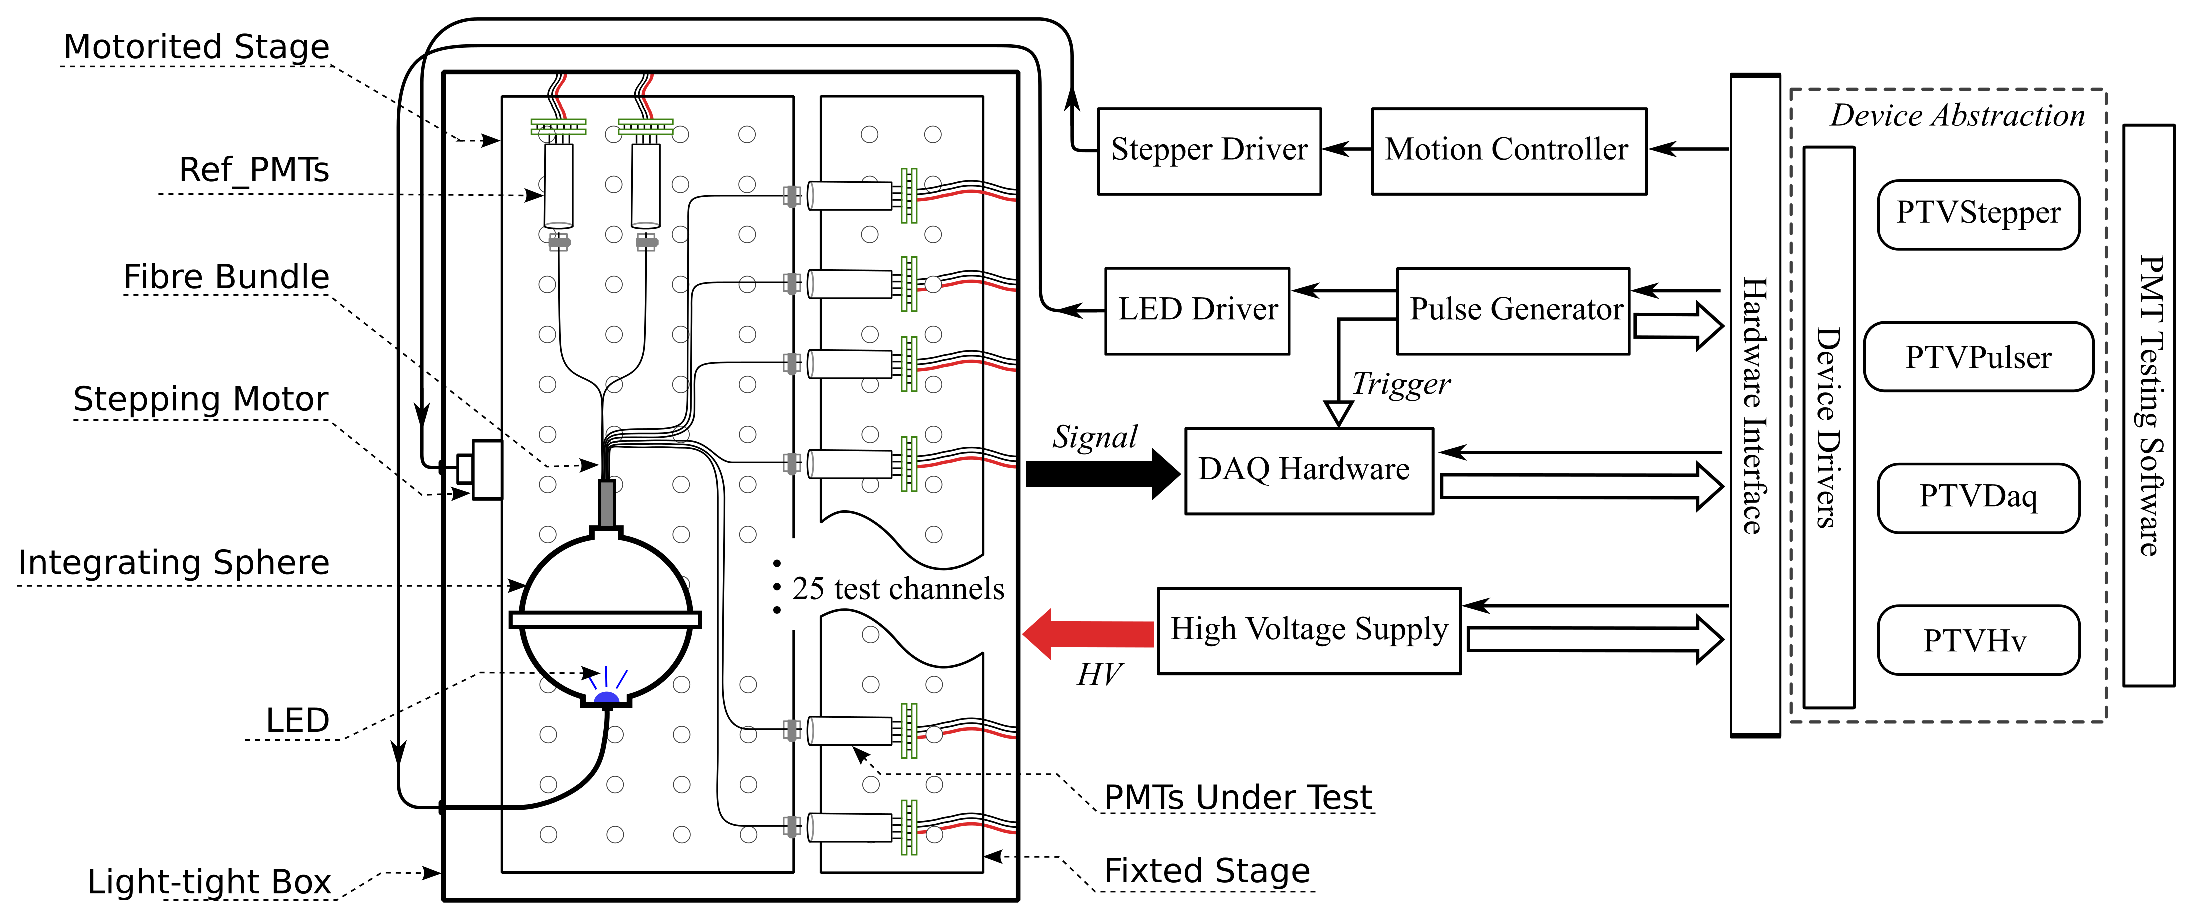
\includegraphics[width=\textwidth]{chap/pmt_test/fig/testbench_schematic.eps}
	\caption{PMT批量测试平台的原理框图}
	\label{fig:pmt_test:testbench_schematic}
\end{figure}

PMT测试平台的大部分辅助设备被都放置在铝合金暗箱的外围,它们与内部器件的连接线缆穿过箱子上不透光的通孔相互联接。
这些辅助设备可以被分为四个不同功能模块,分别为:运动控制模块,光脉冲驱动模块,数据获取模块(简称DAQ模块)以及高压供给模块。
运动控制模块和光驱动模块是和测试平台紧密联系在一起的,而与此相关的设备基本在所有的测试中都可以重复使用。
相反的,DAQ模块和高压供给模块与需要PMT测试的具体项目紧密联系,一般需要使用该项目定制的仪器设备进行测试。
作为一个通用的解决方案,我们为测试平台配备了一个基于CAMAC机箱的DAQ模块以及一个基于CAEN SY1527LC机箱的高压供给模块。
这两个模块可以根据具体情况进行更换,在PSD的PMT性能测试中,我们就将上述CAMAC机箱替换成了PSD专用的地面检测系统(详见\ref{sec:pmt_test:characterization})。

最后,整个PMT测试平台系统被放置在一个十万级的洁净室中,室内温度被控制在$22\pm2$\si{\celsius}。

\subsection{硬件结构与组成}
\label{sec:pmt_test:testbench_hardware}
% 总述硬件结构,之后依次介绍各组件以及相关测试结果。

% 主体平台
\begin{figure}[htbp]
	\centering
	\subfloat[][铝合金暗箱]{
		\label{fig:pmt_test:blackbox}
		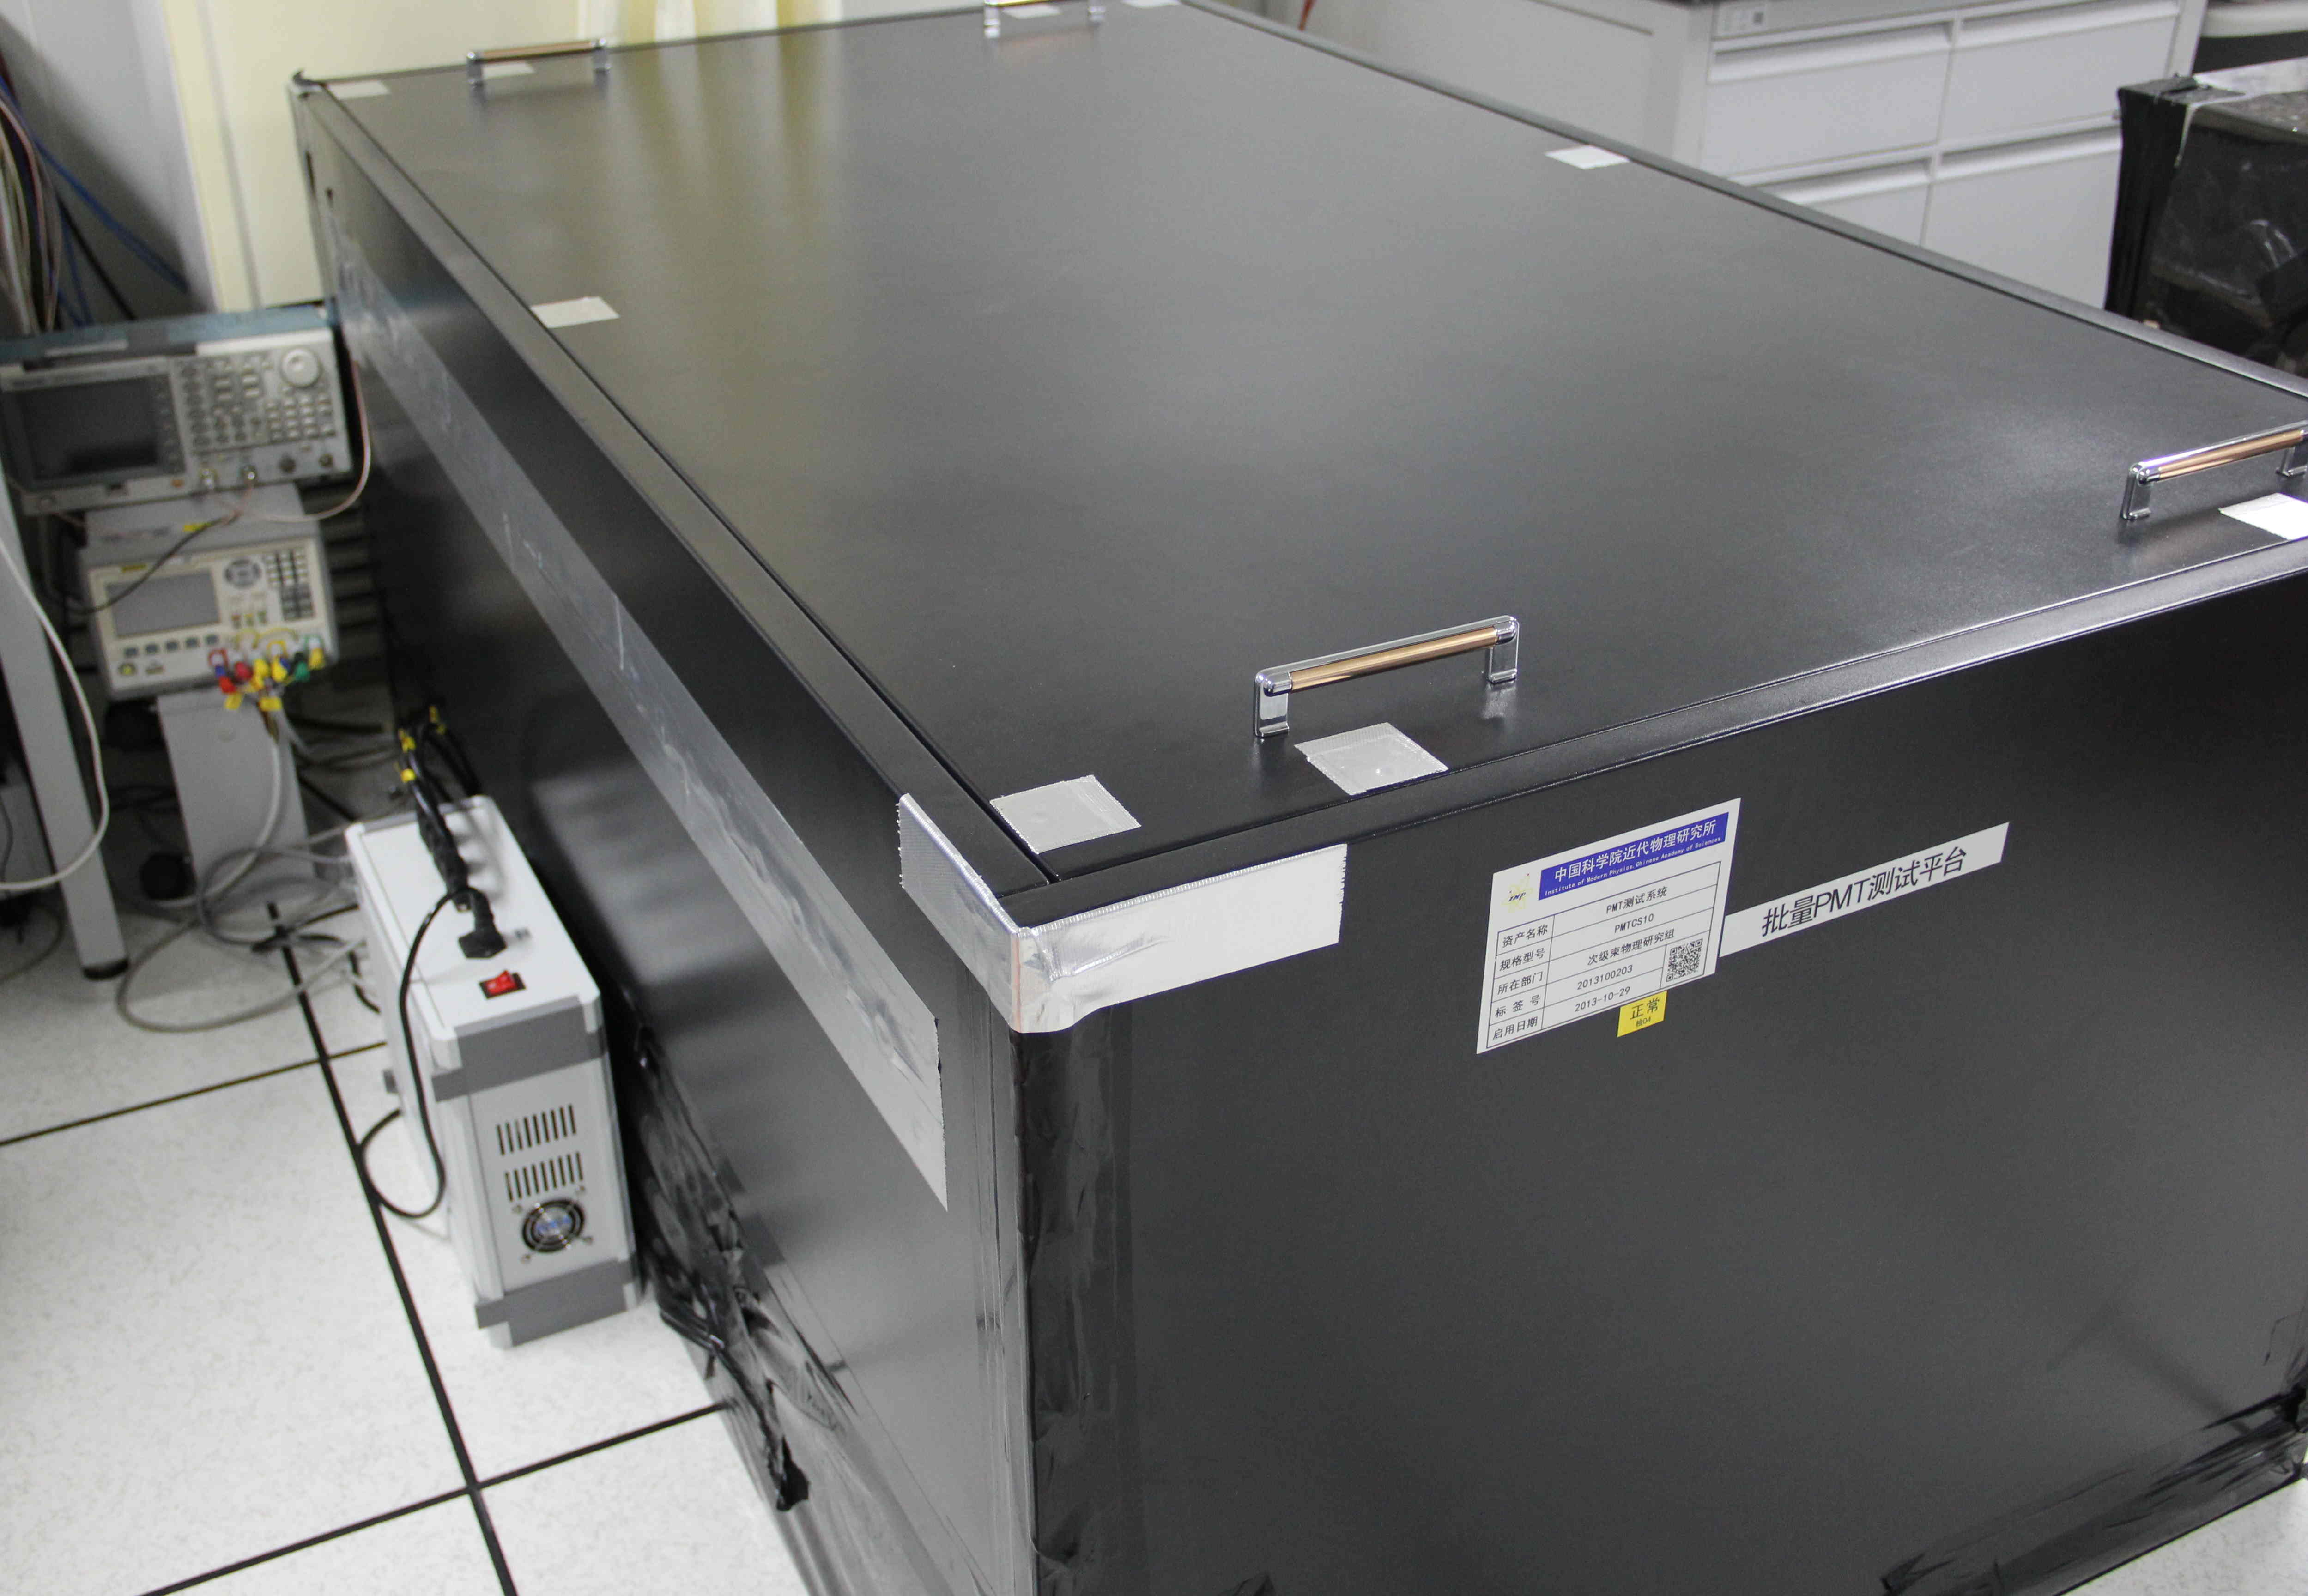
\includegraphics[width=0.49\textwidth]{chap/pmt_test/fig/black_box.jpg}
	}
	\subfloat[][三维移动平台与固定平台]{
		\label{fig:pmt_test:stages}
		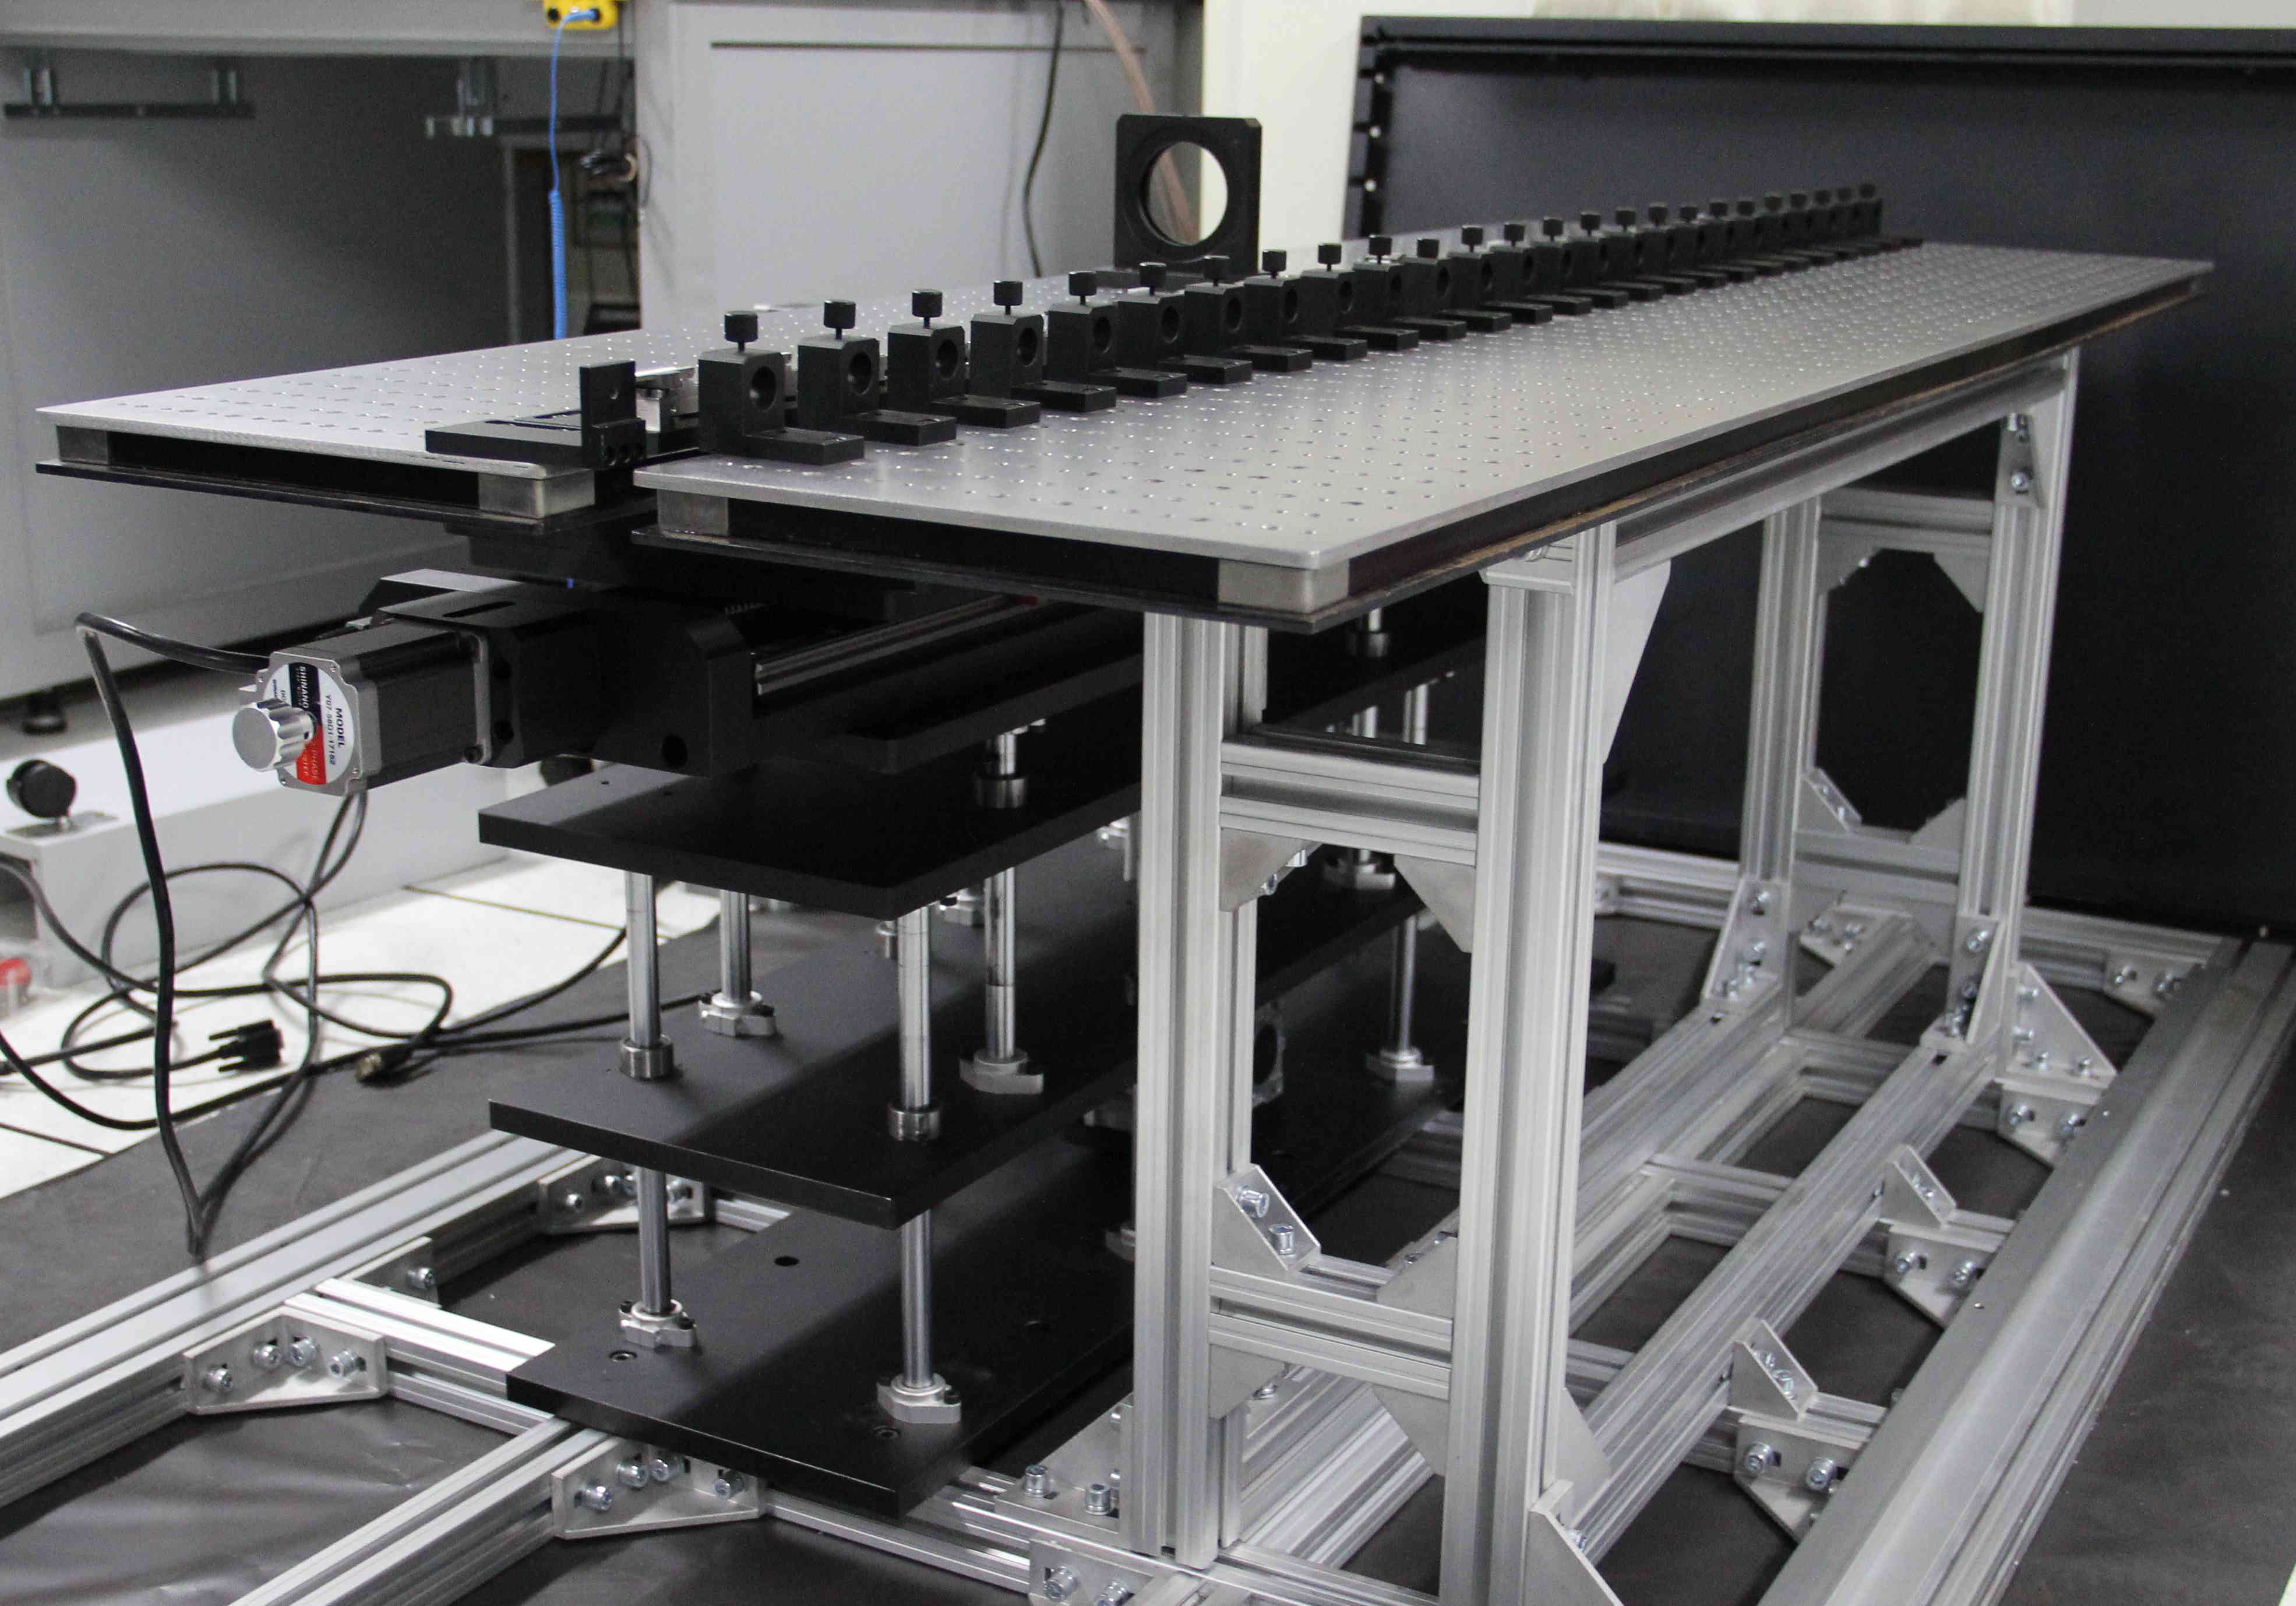
\includegraphics[width=0.49\textwidth]{chap/pmt_test/fig/stages.jpg}
	}
	\caption{PMT批量测试平台的主体结构}
	\label{fig:blindfigure}
\end{figure}

% 紧固件
\begin{figure}[htbp]
	\centering
	\includegraphics[width=0.6\textwidth]{chap/pmt_test/fig/fixtures.jpg}
	\caption{PMT紧固件和光纤紧固件}
	\label{fig:pmt_test:fixtures}
\end{figure}

% 光源
\begin{figure}[htbp]
	\centering
	\subfloat[][1)LED 2)积分球 3)集束光纤]{
		\label{fig:pmt_test:lightsource_components}
		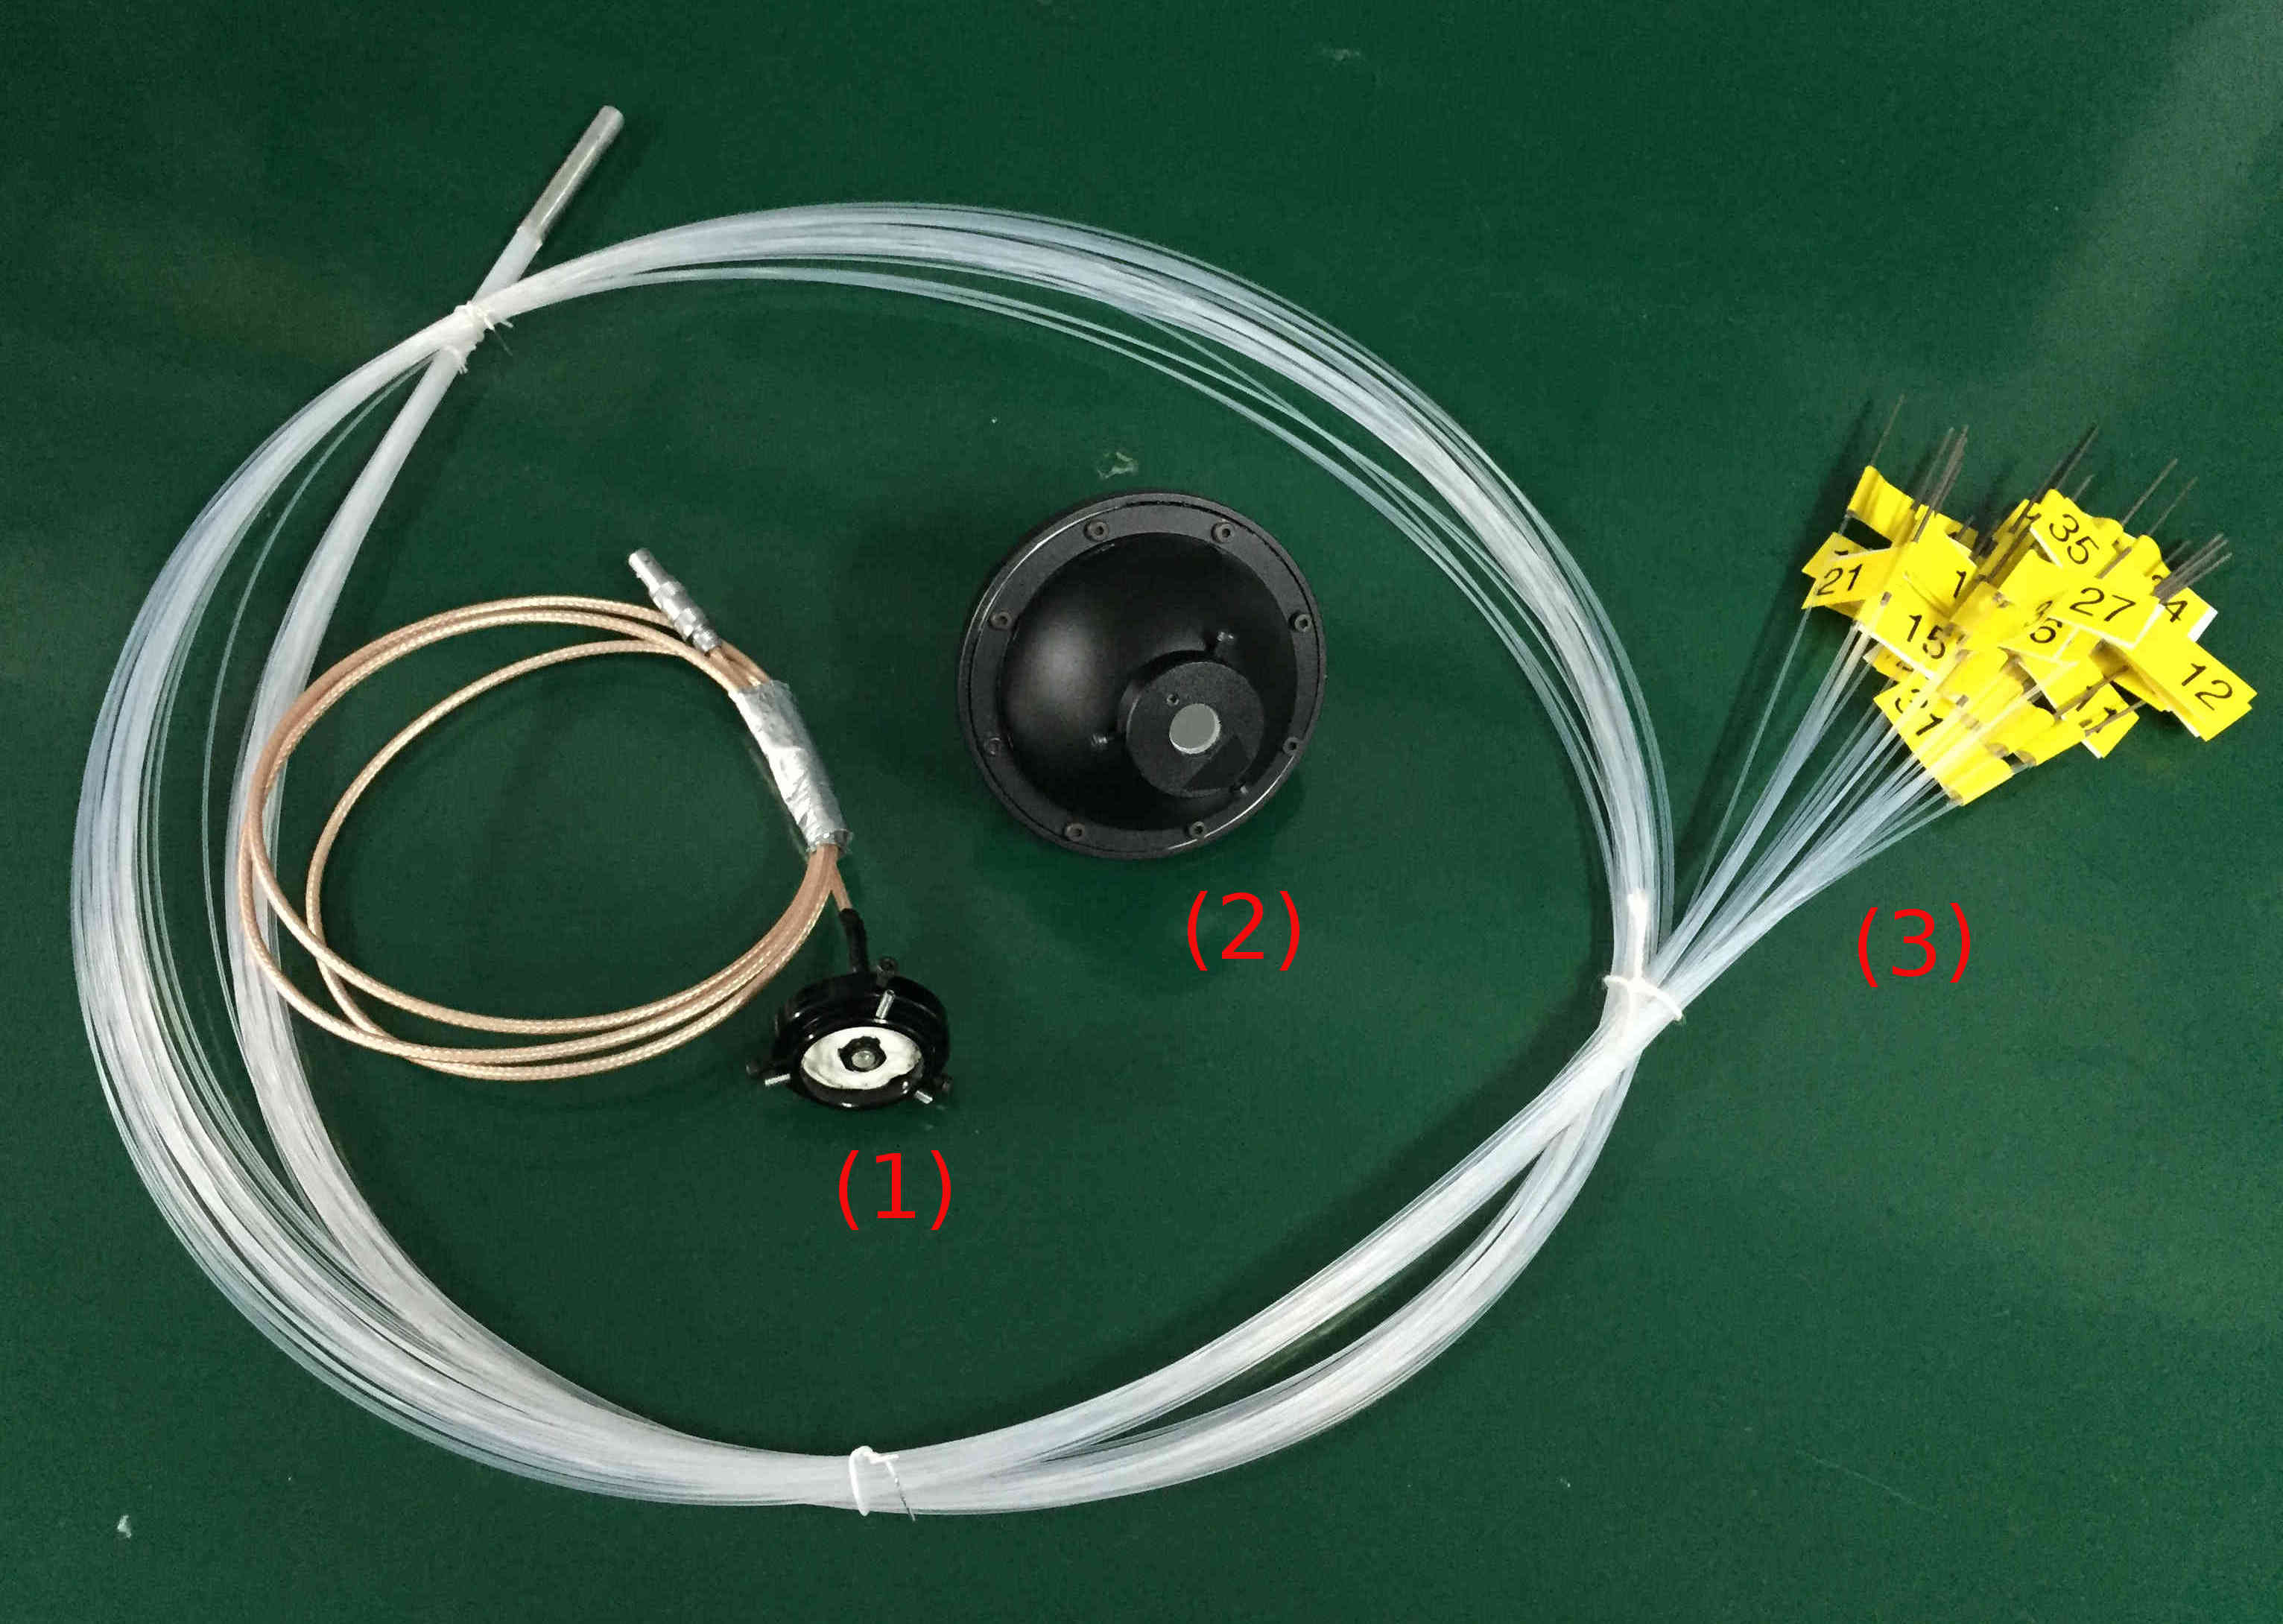
\includegraphics[width=0.49\textwidth]{chap/pmt_test/fig/lightsource_components.jpg}
	}
	\subfloat[][各组件耦合在一起]{
		\label{fig:pmt_test:lightsource_integration}
		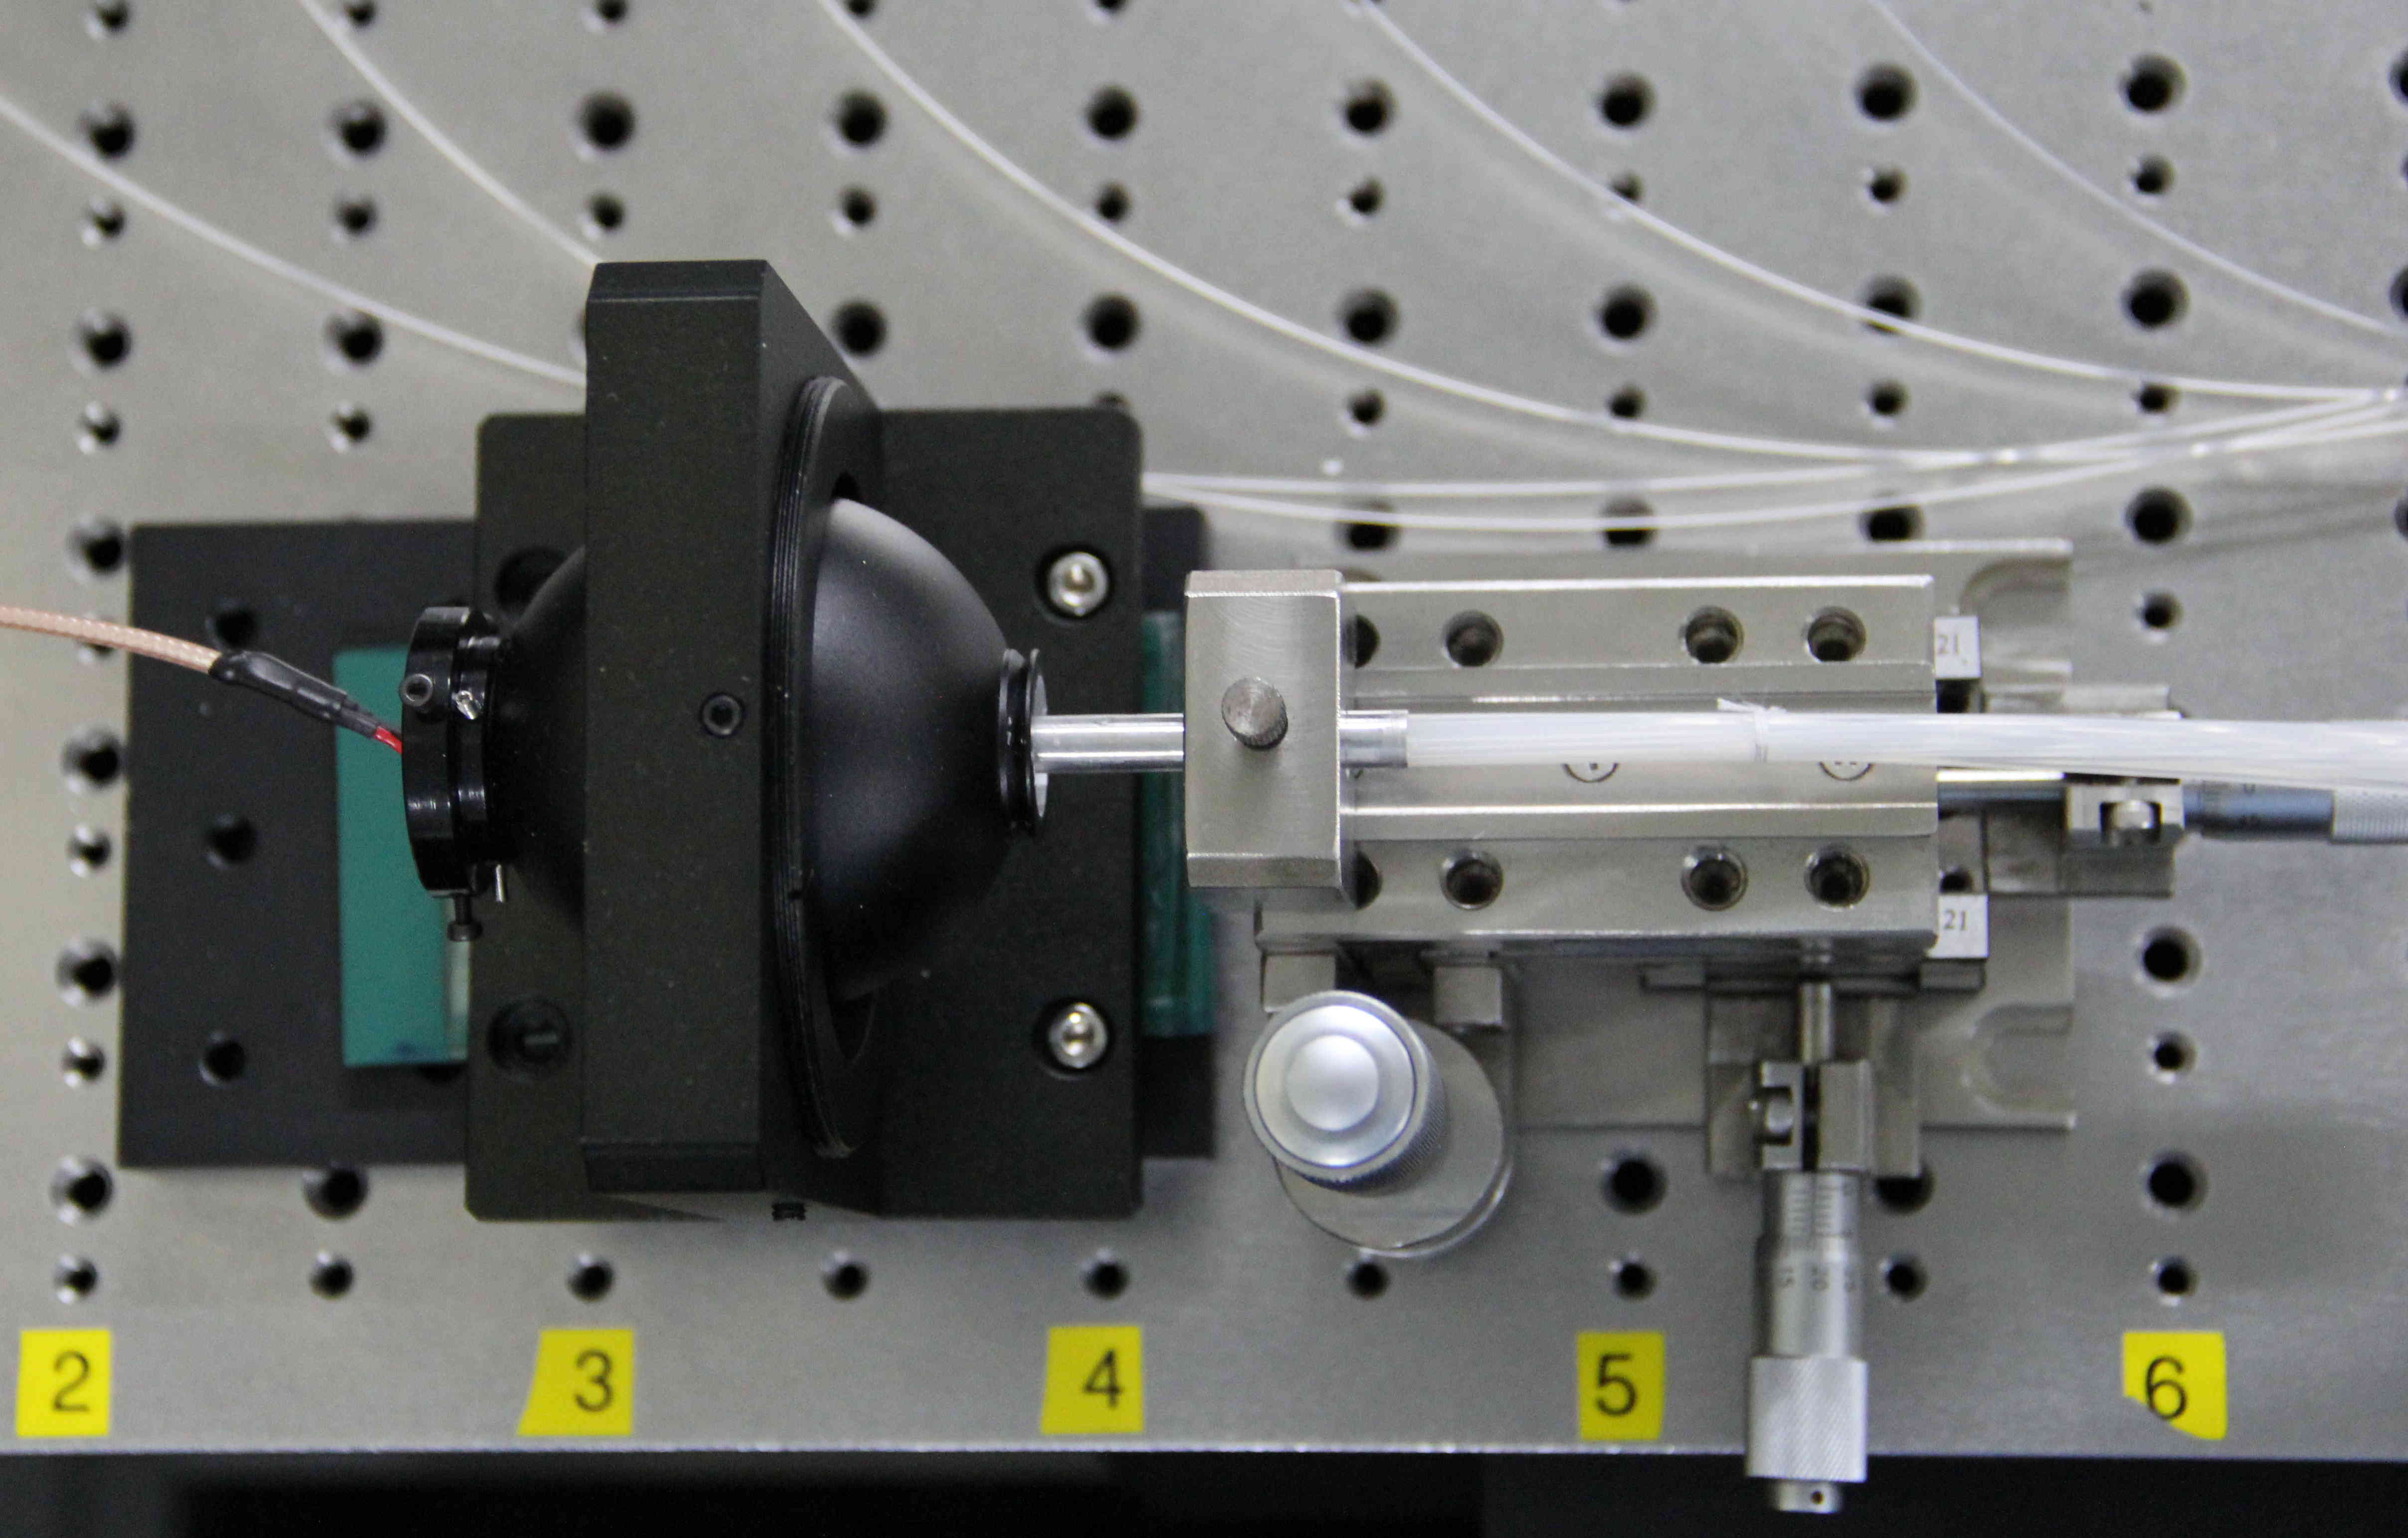
\includegraphics[width=0.49\textwidth]{chap/pmt_test/fig/lightsource_integration.jpg}
	}		
	\caption{PMT批量测试平台的光分配系统}
	\label{fig:pmt_test:light_distribution}
\end{figure}

\begin{figure}[htbp]
	\centering
	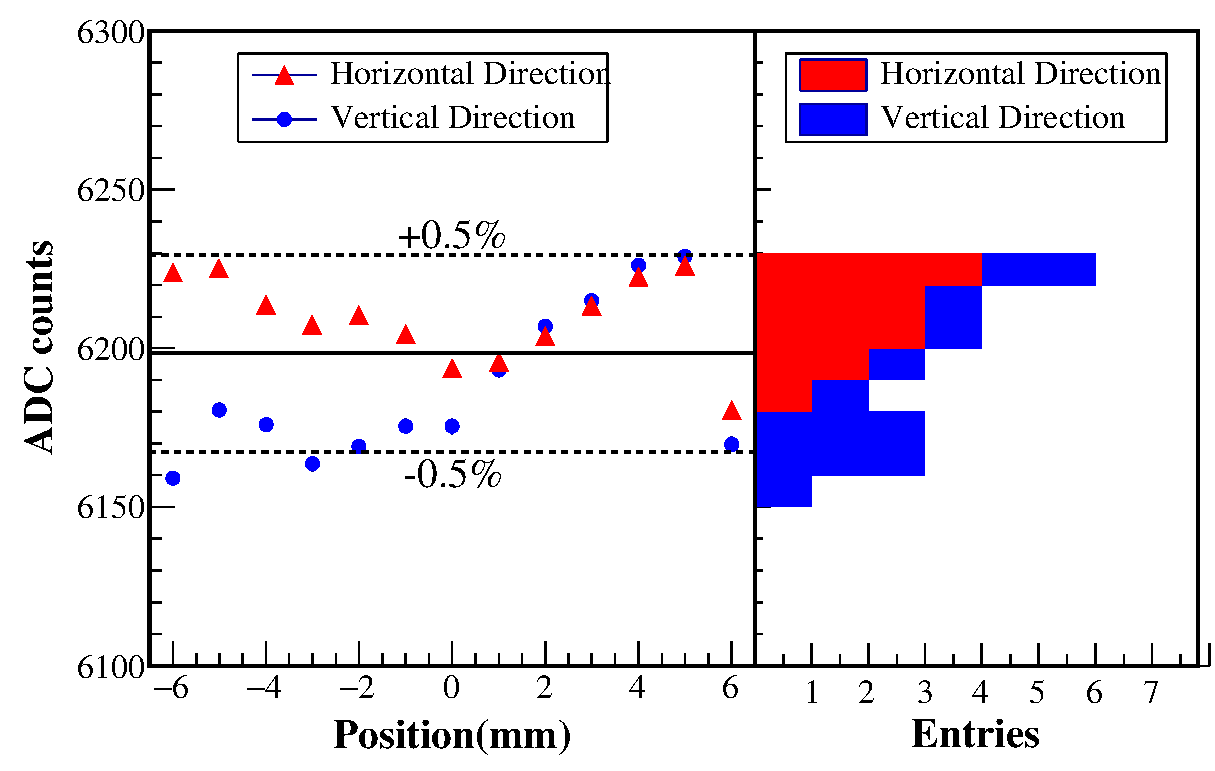
\includegraphics[width=0.65\textwidth]{chap/pmt_test/fig/integrationsphere_uniformity.eps}
	\caption{\SI{5}{cm}铝合金积分球输出端口的光均匀性}
	\label{fig:pmt_test:integrationsphere_uniformity}
\end{figure}

% 光源驱动器
\begin{figure}[htbp]
	\centering
	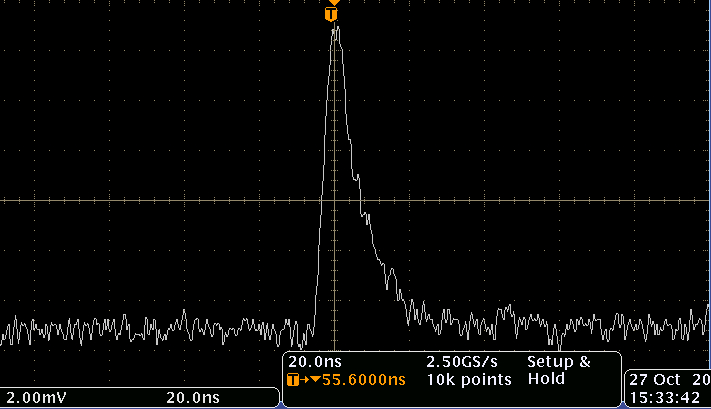
\includegraphics[width=0.65\textwidth]{chap/pmt_test/fig/led_pulse.jpg}
	\caption{输入方波脉冲驱动的LED光得到的R4443原始波形}
	\label{fig:pmt_test:led_pulse}
\end{figure}

\begin{figure}[htbp]
	\centering
	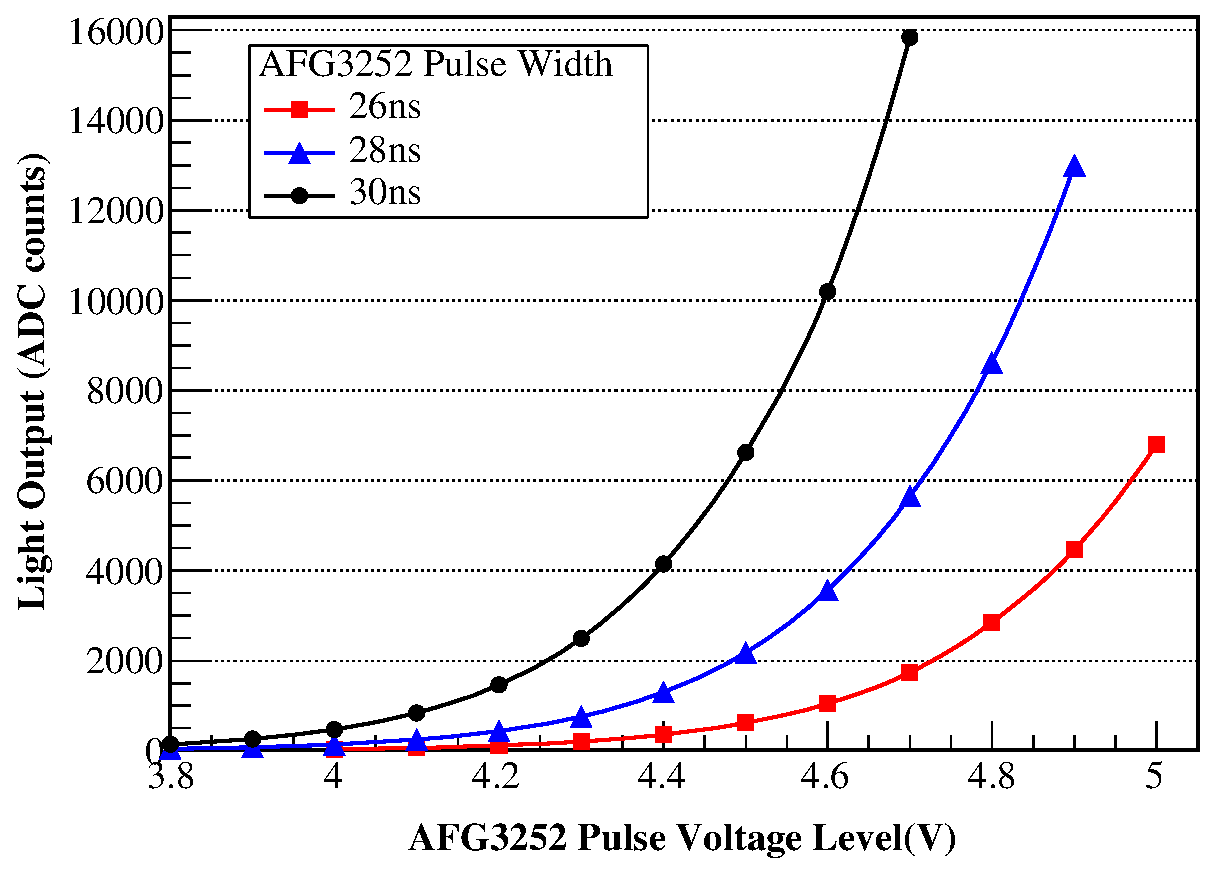
\includegraphics[width=0.62\textwidth]{chap/pmt_test/fig/led_response.eps}
	\caption{LED输出脉冲的光强度与AFG3253脉冲幅度的非线性关系}
	\label{fig:pmt_test:led_response}
\end{figure}

% 集束光纤
\begin{figure}[htbp]
	\centering
	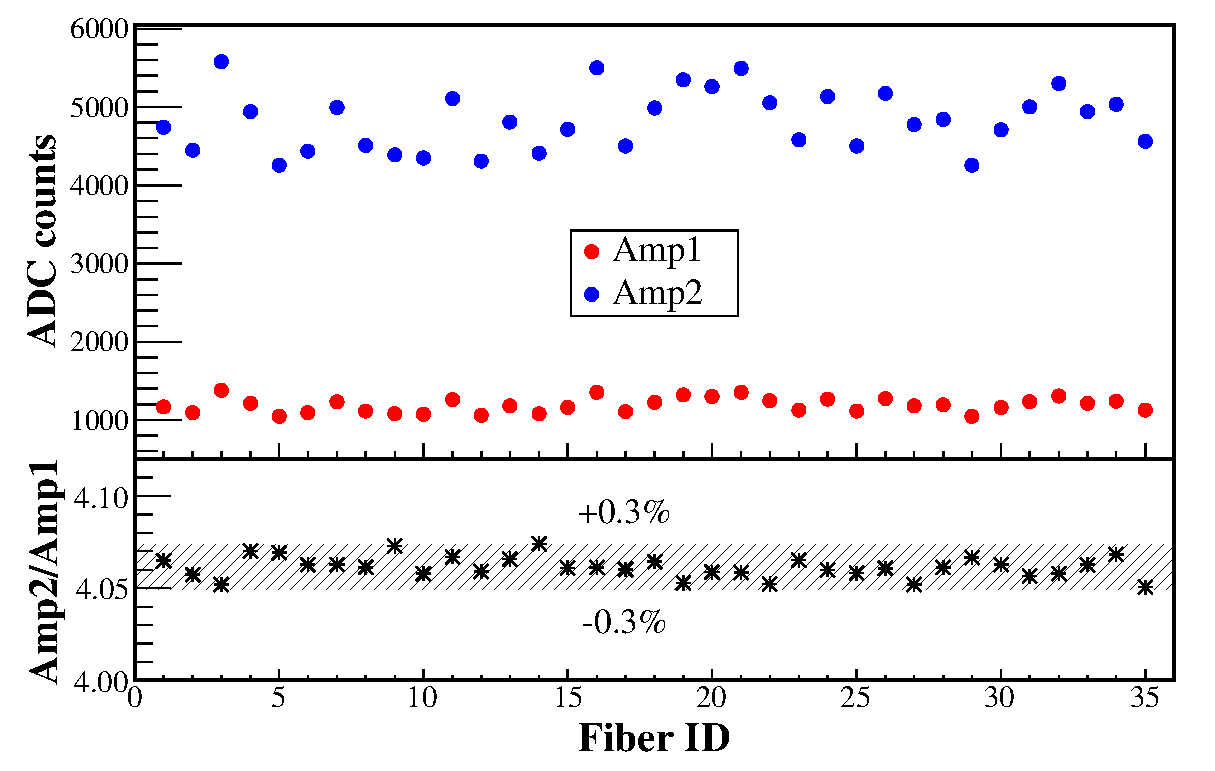
\includegraphics[width=0.7\textwidth]{chap/pmt_test/fig/fiber_difference.eps}
	\caption{集束光纤各通道的光传输差异性}
	\label{fig:pmt_test:fiber_difference}
\end{figure}

\subsection{测控软件}
% 最好这里做一个归纳性的介绍,具体细节设计放到附录中


\section{R4443裸管的性能测试}
\label{sec:pmt_test:characterization}

\subsection{相对增益的测量}
\subsection{Dynode8/Dynode5增益比值的测量}
\subsection{光阴极均匀性}
\subsection{PMT批量测试平台的长期稳定性}

\section{PMT的筛选}

\subsection{筛选方案}
工厂参数。
% 暗电流
PMT的暗电流是指在完全黑暗且没有入射光的条件下,在光电倍增管内部流动的微小电流。
由于暗电流会使得探测器的基线展宽、噪声变大,严重的情况下甚至降低探测器的能量分辨率,因此暗电流越小越好。
光电倍增管的光阴极材料是引起暗电流的主要因素。
PSD采用的R4443型号(即MOD2)使用低噪声的碱金属材料作为光阴极,从而极大地抑制了暗电流的大小。
根据Hamamatsu提供的出厂测试信息,我们发现所有管子的暗电流都小于PSD的要求。
% 增益
R4443的Dy8通道用于覆盖PSD动态范围的低端部分,主要用于$e/\gamma$;R4443的Dy5通道用于覆盖PSD动态范围的高端部分,主要用于相对论重离子的电荷测量。
我们希望Dy8的增益尽量高,使其测得的MIP信号尽量与基线噪声相分离,从而降低$e/\gamma$误判率。
另一方面,PSD对整体的动态范围有严格的区间要求($\SI{0.1}{MIPs}\sim\SI{1400}{MIPs}$),过高的Dy8增益会压低Dy5的增益(即提高了Dy58比值),从而降低Dy5对重离子电荷的分辨能力。
因此
\subsection{参考单元模块的MIPs响应}
\subsection{与塑闪单元条的匹配}